\subsubsection{Subsystem Overview}
The computing platform's power subsystem consists of a commercially produced integrated battery and power management pack. The devices powered by this subsystem include the:

\begin{itemize}
\item Platform Management Board (Raspberry Pi) -- maximum current draw of 1.2 A and a typical current draw of 0.4 A, and
\item Programmable Logic Board (Zedboard) -- maximum current draw of 1 A and a typical current draw of 0.4 A
\end{itemize}

The power system must provide continuous power to the computing platform for at least 20 minutes (\textbf{F.PR.1}).

\subsubsection{Seperate vs Common Power Supplies}
Two power supply schemes were considered for the device: a common power supply shared between the multirotor and the computing platform, or separate power supplies across the two systems. While separating the power systems adds complexity and weight, it provides the following benefits:

\begin{itemize}
    \item No risk of noise from the motors interfering with the computational hardware.
    \item Allows for testing of the computational hardware separately from the drone.
    \item Reduces the difficulty of replacing the multirotor assembly, if required.
\end{itemize}

Ultimately it was determined that the advantages of using separate power supplies, in particular, avoiding motor noise, warranted the extra weight and complexity.

\subsubsection{Custom vs Commercial Power Bank}
Initially a custom designed power supply system was intended to be used. It was to consist of a lithium-polymer or lithium-ion battery and a battery management system. Such a battery management system (seen in Figure \ref{powerdiag}) would consist of two DC-DC converters (with an approximate efficiency of 94\%), a battery protection board, and a battery monitor. 

\begin{figure}[H]
\centering
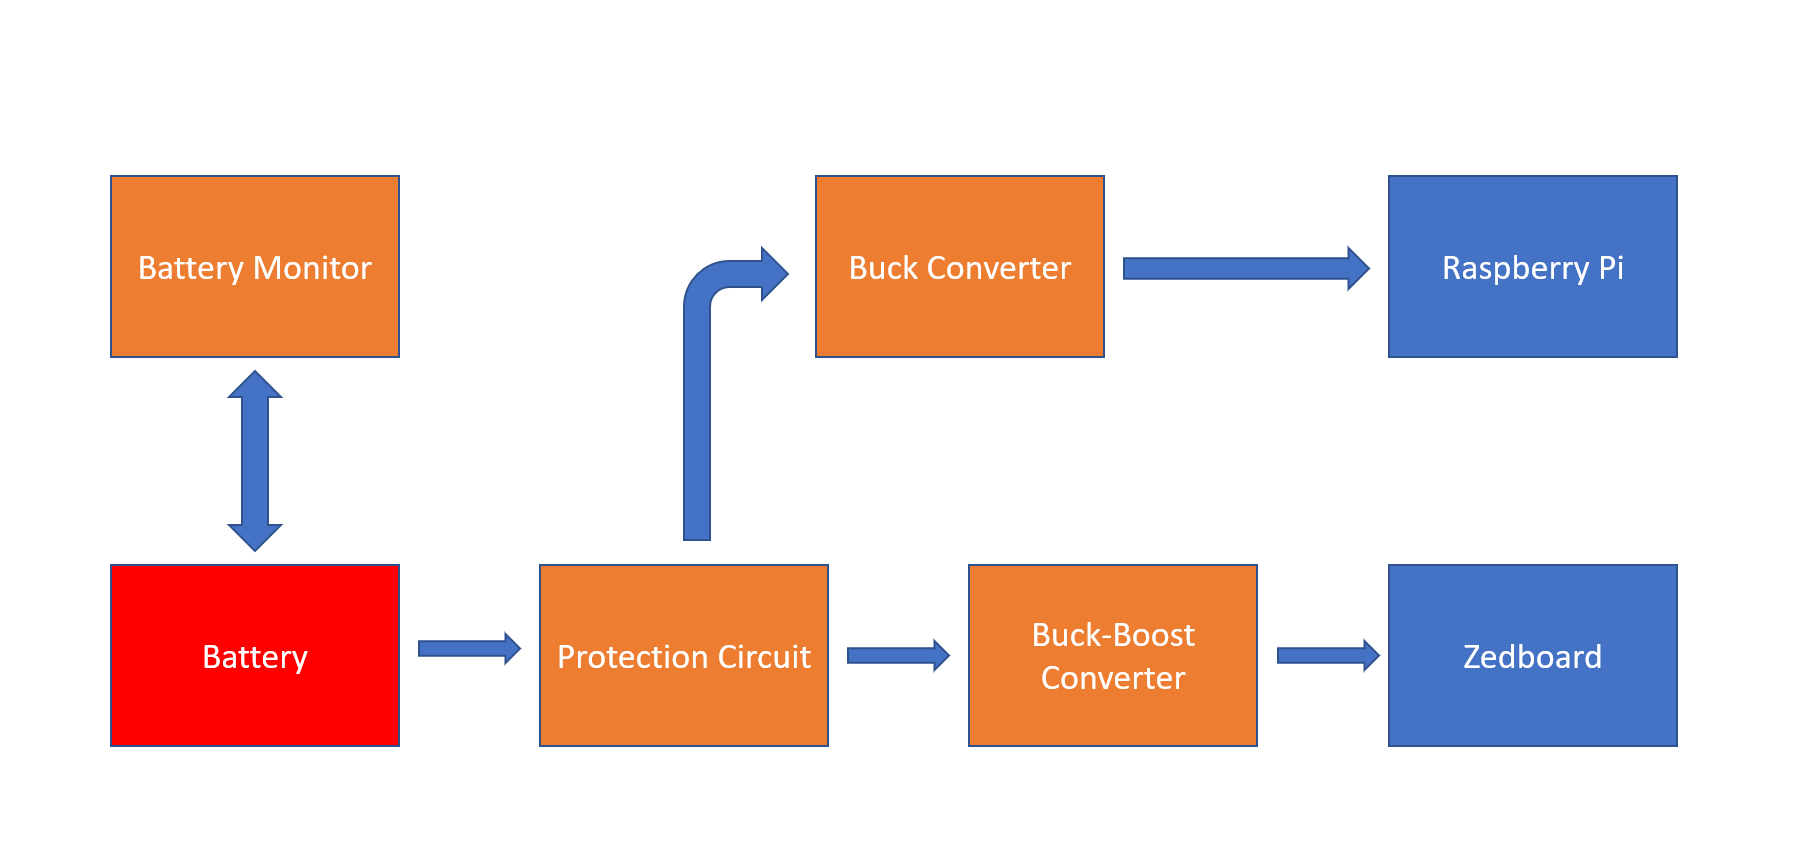
\includegraphics[width=15cm]{img/Power_Diagram.png}
\caption{Original Custom-Designed Computing Power System}
\label{powerdiag}
\end{figure}

Using a custom designed power supply, DC-DC conversion would have been accomplished through use of a buck converter for the 5V output and a buck-boost converter for the 12V output.

\begin{figure}[H]
\centering
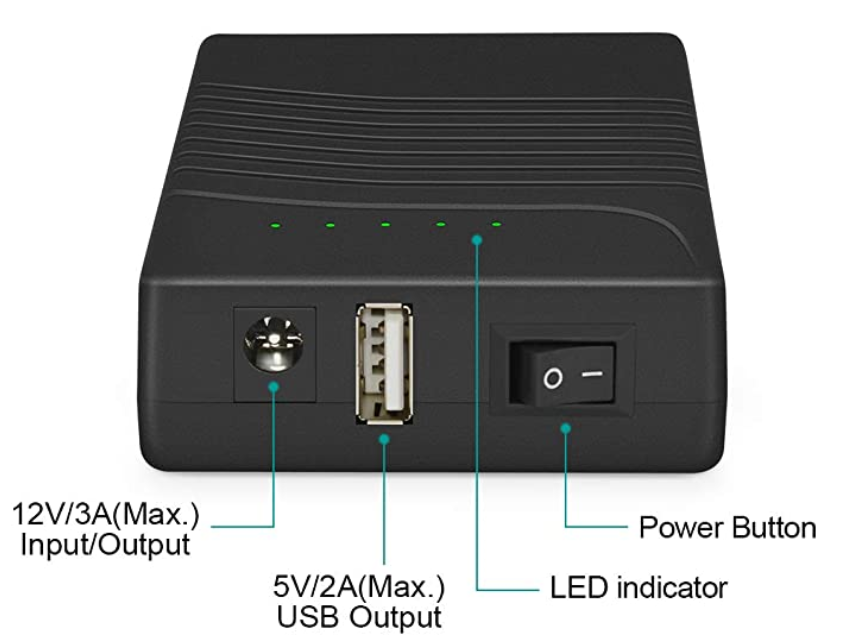
\includegraphics[width=12cm]{img/power_bank.png}
\caption{Commercial Power Bank}
\label{powerbank}
\end{figure}

After designing the system, an alternative commercial power bank was found which fits the project requirements (see Figure \ref{powerbank}). This commercial power bank consists of 3 lithium-ion batteries with a combined capacity of 3000mAh in addition to a power management circuit. The power bank provides a 5V/2A USB output port and a 12V/3A output port which are compatible with the Raspberry Pi and the Zedboard respectively. The rated maximum current output from each port is sufficient to simultaneously supply both computation boards, and the battery capacity is rated to provide 3 hours and 45 minutes of operation on a single charge.

Ultimately, we chose the commercial power bank for its lower cost and smaller form factor.
